% ----------------------------------------------------
% Sensing Subsystem
% ----------------------------------------------------
\documentclass[class=report,11pt,crop=false]{standalone}
% Page geometry
\usepackage[a4paper,margin=20mm,top=25mm,bottom=25mm]{geometry}

% Font choice
\usepackage{lmodern}

\usepackage{lipsum}

% Use IEEE bibliography style
\bibliographystyle{IEEEtran}

% Line spacing
\usepackage{setspace}
\setstretch{1.20}

% Ensure UTF8 encoding
\usepackage[utf8]{inputenc}

% Language standard (not too important)
\usepackage[english]{babel}

% Skip a line in between paragraphs
\usepackage{parskip}

% For the creation of dummy text
\usepackage{blindtext}

% Math
\usepackage{amsmath}

% Header & Footer stuff
\usepackage{fancyhdr}
\pagestyle{fancy}
\fancyhead{}
\fancyhead[R]{\nouppercase{\rightmark}}
\fancyfoot{}
\fancyfoot[C]{\thepage}
\renewcommand{\headrulewidth}{0.0pt}
\renewcommand{\footrulewidth}{0.0pt}
\setlength{\headheight}{13.6pt}

% Epigraphs
\usepackage{epigraph}
\setlength\epigraphrule{0pt}
\setlength{\epigraphwidth}{0.65\textwidth}

% Colour
\usepackage{color}
\usepackage[usenames,dvipsnames]{xcolor}

% Hyperlinks & References
\usepackage{hyperref}
\definecolor{linkColour}{RGB}{77,71,179}
\hypersetup{
    colorlinks=true,
    linkcolor=linkColour,
    filecolor=linkColour,
    urlcolor=linkColour,
    citecolor=linkColour,
}
\urlstyle{same}

% Automatically correct front-side quotes
\usepackage[autostyle=false, style=ukenglish]{csquotes}
\MakeOuterQuote{"}

% Graphics
\usepackage{graphicx}
\graphicspath{{Images/}{../Images/}}
\usepackage{makecell}
\usepackage{transparent}

% SI units
\usepackage{siunitx}

% Microtype goodness
\usepackage{microtype}

% Listings
\usepackage[T1]{fontenc}
\usepackage{listings}
\usepackage[scaled=0.8]{DejaVuSansMono}

% Custom colours for listings
\definecolor{backgroundColour}{RGB}{250,250,250}
\definecolor{commentColour}{RGB}{73, 175, 102}
\definecolor{identifierColour}{RGB}{196, 19, 66}
\definecolor{stringColour}{RGB}{252, 156, 30}
\definecolor{keywordColour}{RGB}{50, 38, 224}
\definecolor{lineNumbersColour}{RGB}{127,127,127}
\lstset{
  language=Matlab,
  captionpos=b,
  aboveskip=15pt,belowskip=10pt,
  backgroundcolor=\color{backgroundColour},
  basicstyle=\ttfamily,%\footnotesize,        % the size of the fonts that are used for the code
  breakatwhitespace=false,         % sets if automatic breaks should only happen at whitespace
  breaklines=true,                 % sets automatic line breaking
  postbreak=\mbox{\textcolor{red}{$\hookrightarrow$}\space},
  commentstyle=\color{commentColour},    % comment style
  identifierstyle=\color{identifierColour},
  stringstyle=\color{stringColour},
   keywordstyle=\color{keywordColour},       % keyword style
  %escapeinside={\%*}{*)},          % if you want to add LaTeX within your code
  extendedchars=true,              % lets you use non-ASCII characters; for 8-bits encodings only, does not work with UTF-8
  frame=single,	                   % adds a frame around the code
  keepspaces=true,                 % keeps spaces in text, useful for keeping indentation of code (possibly needs columns=flexible)
  morekeywords={*,...},            % if you want to add more keywords to the set
  numbers=left,                    % where to put the line-numbers; possible values are (none, left, right)
  numbersep=5pt,                   % how far the line-numbers are from the code
  numberstyle=\tiny\color{lineNumbersColour}, % the style that is used for the line-numbers
  rulecolor=\color{black},         % if not set, the frame-color may be changed on line-breaks within not-black text (e.g. comments (green here))
  showspaces=false,                % show spaces everywhere adding particular underscores; it overrides 'showstringspaces'
  showstringspaces=false,          % underline spaces within strings only
  showtabs=false,                  % show tabs within strings adding particular underscores
  stepnumber=1,                    % the step between two line-numbers. If it's 1, each line will be numbered
  tabsize=2,	                   % sets default tabsize to 2 spaces
  %title=\lstname                   % show the filename of files included with \lstinputlisting; also try caption instead of title
}

% Caption stuff
\usepackage[hypcap=true, justification=centering]{caption}
\usepackage{subcaption}

% Glossary package
% \usepackage[acronym]{glossaries}
\usepackage{glossaries-extra}
\setabbreviationstyle[acronym]{long-short}

% For Proofs & Theorems
\usepackage{amsthm}

% Maths symbols
\usepackage{amssymb}
\usepackage{mathrsfs}
\usepackage{mathtools}

% For algorithms
\usepackage[]{algorithm2e}

% Spacing stuff
\setlength{\abovecaptionskip}{5pt plus 3pt minus 2pt}
\setlength{\belowcaptionskip}{5pt plus 3pt minus 2pt}
\setlength{\textfloatsep}{10pt plus 3pt minus 2pt}
\setlength{\intextsep}{15pt plus 3pt minus 2pt}

% For aligning footnotes at bottom of page, instead of hugging text
\usepackage[bottom]{footmisc}

% Add LoF, Bib, etc. to ToC
\usepackage[nottoc]{tocbibind}

% SI
\usepackage{siunitx}

% For removing some whitespace in Chapter headings etc
\usepackage{etoolbox}
\makeatletter
\patchcmd{\@makechapterhead}{\vspace*{50\p@}}{\vspace*{-10pt}}{}{}%
\patchcmd{\@makeschapterhead}{\vspace*{50\p@}}{\vspace*{-10pt}}{}{}%
\makeatother
\makenoidxglossaries

\newacronym{radar}{RADAR}{Radio Detection and Ranging}
\begin{document}
	% ----------------------------------------------------
	\chapter{Sensing Subsystem (NXSMPI001)}
	\vspace{0.5cm}
	% ----------------------------------------------------
	\section{Introduction}
	The aim of this subsystem is to translate the force from the bird's weight on the scale into a digital reading. It involves designing and constructing the circuitry needed to change the weight into a analogue voltage, developing the algorithms in the micro-controller unit (MCU) used to process this signal and change it into a weight reading of the bird. Another component to this subsystem is to have accurate timekeeping so the weight data is timestamped. 
	
	\section{Requirements Analysis}
	\begin{table}[h!]
		\centering
		\caption{Non-functional Specifications of the Sensing Subsystem}
		\label{tab:S1}
			\begin{tabularx}{0.8\textwidth}{ 
					| >{\centering\arraybackslash}m 
					| >{\centering\arraybackslash}b 
					| >{\centering\arraybackslash}s |}
			\hline
			\textbf{User   Requirement} & \textbf{Specification   Description}                                     & \textbf{Specification   no.} \\ \hline
			Portable                    & The final   circuitry must be able to fit in a box that is 100x100x50mm. & SS1                          \\ \hline
			Long battery   life         & The final   circuitry should consume less than 30mA.                     & SS2                          \\ \hline
			\end{tabularx}
	\end{table}
	
	\begin{table}[h!]
		\centering
		\caption{Functional Specifications for Sensing Subsystem}
		\label{tab:S2}
			\begin{tabularx}{0.8\textwidth}{ 
					| >{\centering\arraybackslash}m 
					| >{\centering\arraybackslash}b 
					| >{\centering\arraybackslash}s |}
				\hline
				\textbf{User   Requirement}                                   & \textbf{Specification   Description}                                                                                                             & \textbf{Specification   no.} \\ \hline
				The scale   must measure weights of up to 500g.               & The weight   sensor must have a maximum capacity greater than 750g (1.5 times safety   factor).                                                  & SS3                          \\ \hline
				& The sensor   and amplifier must output a voltage proportional to the weight force applied   up to a weight of 500g.                              & SS4                          \\ \hline
				& Microcontroller must have an algorithm for converting output codes from the ADC into a weight measurement.                                                             & SS5                          \\ \hline
				\multirow{2}{0.2\textwidth}{The scale   measure weight accurate to 0.1g.} & The ADC must   be able to resolve voltage changes from weight changes that are less than   0.1g.                                                 & SS6                          \\ \cline{2-3} 
				& The ADC must   have a gain and offset error less than a voltage change resulting from a   change in weight of 0.1g.                              & SS7                          \\ \hline
				\multirow{3}{0.2\textwidth}{The scale   must have a tare function to ignore the weight of the perch}        & The   microcontroller must have a digital input pin to read the user's inputs.                                               & SS8                          \\ \cline{2-3} 
				& The microcontroller must subtract the current weight from all subsequent measurements when the digital pin receives an input. & SS9                          \\ \cline{2-3} 
				& There must be   an LED that indicates when the scale is in tare mode.                                                                            & SS10                         \\ \hline
				The scale must   be battery powered.                          & The microcontroller   and all the surrounding circuitry must be able to operate with one positive   rail.                                          & SS11                         \\ \hline
			\end{tabularx}
	\end{table}
	
	\section{Design Process}
	
	\subsection{Microcontroller Unit (MCU)}
	The Arduino was chosen as its Integrated Development Environment (IDE) has ample support and libraries which will make interfacing with all different modules simple and straightforward. Within the Arduino family the Arduino Nano was initially chosen as it was one of the cheapest Arduino and it came in a small form factor. However, the User Interface subsystem required a WiFi or Bluetooth module so the Arduino Nano 33 IoT was chosen instead. Although BLE and BLE Sense also meet these requirements, they come with additional sensors that are unnecessary. All the Arduino chips also come with several low power modes that can be leveraged to reduce power consumption.
	
	\subsection{Weight Sensor}
	A strain gauge is an electrical component whose resistance changes when a force is applied to it. Strain gauges work on the principle that when the resistance of a conductor is proportional to its length, as shown in the equation below. 
	\[R = \rho \frac{L}{A}\]
	One solution is to put a strain gauge in series with another resistance, then place the strain gauge on a beam. When the beam deflects under the bird’s weight, the change in voltage across the strain gauge can be measured. The issue with this setup is that the change in resistance, and thus the subsequent change in voltage, will be very small. This means a very high resolution ADC will be required to resolve these small changes in voltage. The resolution required could be reduced by amplifying the signal, however this would also amplify the DC offset introduced by the voltage divider, quickly saturating the output.
	
	A better solution is a load cell which has 4 strain gauges in a Wheatstone configuration. This means that when the load cell has no load on it, the voltage will be zero, and when the device deflects, there will be a slight voltage difference between it’s 2 output terminals. As discussed above, this output can be sent through an amplifier thus reducing the resolution required for the ADC. To meet the sensor specifications, a 1kg load cell will be used. 
	
	The specifications for one such load cell by HKD is shown in Table \ref{tab:S3} below.

	\begin{table}[h!]
		\centering
		\caption{Table on load cell specifications}
		\begin{tabularx}{0.8\textwidth} { 
				| >{\centering\arraybackslash}X 
				| >{\centering\arraybackslash}X |}
			\hline
			Rated Load & 1kg \\
			\hline
			Rated Output & 1.0 ± 0.15mV/V \\
			\hline
			Zero Output & ±0.1mV/V \\
			\hline
			Input Impedance & 1115 ± 10$\Omega$ \\
			\hline
			Output Impedance & 1000 ± 10$\Omega$ \\
			\hline
		\end{tabularx}
		\label{tab:S3}
	\end{table}
	
	At the rated load, the output will be $0.001V_{cc}$, hence the amplifier needs a gain of 1000. 
	
	\subsection{Sensor Amplifier}
	From Table \ref{tab:S3}, the output impedance of the load cell is quite significant, meaning there will need to be an input buffer between it and the amplifier to avoid loading. The instrumentation amplifier is thus ideal circuit for achieving this and it is shown in Figure \ref{fig:S1} below.
	
	\begin{figure}[h!]
		\centering
		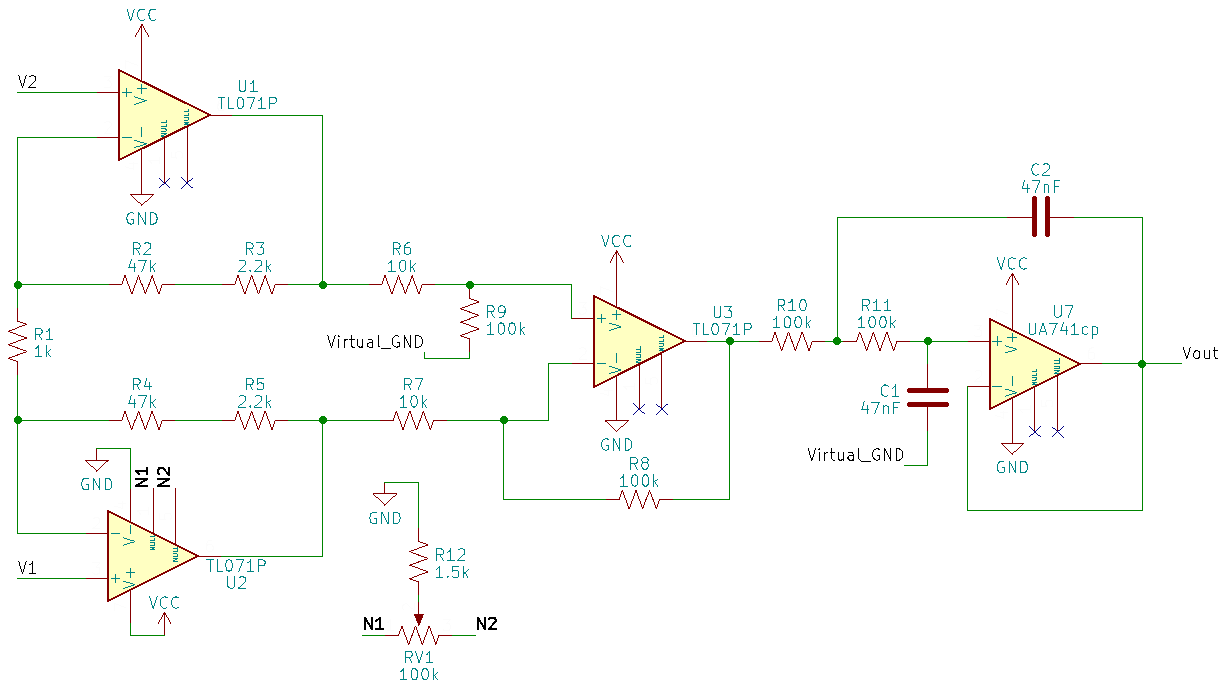
\includegraphics[width=0.9\linewidth]{Figures/Amplifier.png}
		\caption{Circuit Schematic of Instrumentation Amplifier}
		\label{fig:S1}
	\end{figure}
	
	The circuit has three stages. The first stage has two input buffers which also amplify the input signal. The second is a differential amplifier which is a circuit whose output is proportional to the difference between the two inputs. The final stage is a low pass filter. The final output voltage is related to the input voltage by the expression below.
	\[V_{out} = (V_2 - V_1) \left(1 + \frac{2(R_2+R_3)}{R_1}\right) \left(\frac{R_9}{R_6}\right) \]
	From the expression above, when the load cell is connected to the two input terminals, its output will be amplified by a factor of 994, which is close to the gain required. 
	The amplifier have such a large gain presents two issues.
	
	The first is that real op-amps have an input offset voltage. As the offsets from the input stage propagate through the circuit, they are amplified resulting in the output having a large bias and saturating for very small weights, hence the op-amps used were the TL071P. These are JFET op-amps meaning they have a very low input offset voltage, in this case, of 1mV. This is still large in comparison to the input, but they also come with two NULL pins which allows the input offset to be adjusted, and thus reduced to 0. The is the purpose of potentiometer RV1 in Figure \ref{fig:S1}. Another reason for choosing TL071P is that their minimum recommended supply voltage is 4.5V which means unlike other JFET op-amps they can operate at lower supply voltages. This advantageous since the scale will be battery powered so there will not be a large supply.
	
	The second is that noise from the input will also be amplified as it propagates through circuit, making the final output difficult to measure. The low pass filter in the final stage addresses this. Since output is a DC voltage, ideally the cutoff frequency should be as low as possible to attenuate the most amount of noise, but this would have a negative impact on the rise time. A lower cutoff frequency would also require larger capacitors. The sample rate for final system will be 10Hz (discussed later). This equates to a period of 0.1s and ideally the output should settle within half that time. It takes 5 time constants for the output to settle to 99\% of its final value. This means that $5RC = 0.05s$ or $RC = 0.01s$. If a 100k$\Omega$ resistor is used then the capacitor would need 100nF. The filter also needs a steep roll-off to ensure a clean output, so a second stage can be added at the input, to make it a second order filter. The input stage of this filter needs to have much lower impedance than output stage to avoid loading, which would resulting in the filter having a larger cutoff frequency than was calculated. Using a 10k$\Omega$ resistor, the capacitor needed would be 1uF. The equates to a cutoff frequency of 16Hz. It is difficult to know the exact rise time for higher order filters from calculation alone, as such, this filter was simulated in LTSpice. The circuit diagram is shown in Figure \ref{fig:S2} below.
	
	\begin{figure}[h!]
		\centering
		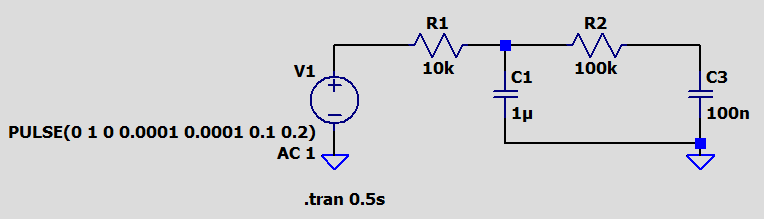
\includegraphics[width=0.5\linewidth]{Figures/Filter.png}
		\caption{Circuit Schematic of Low Pass Filter}
		\label{fig:S2}
	\end{figure}
	
	The input was set to a 1$V_{pp}$ square wave with a frequency of 5Hz. Figure \ref{fig:S3} below shows the input and output of the circuit.
	
	\begin{figure}[h!]
		\centering
		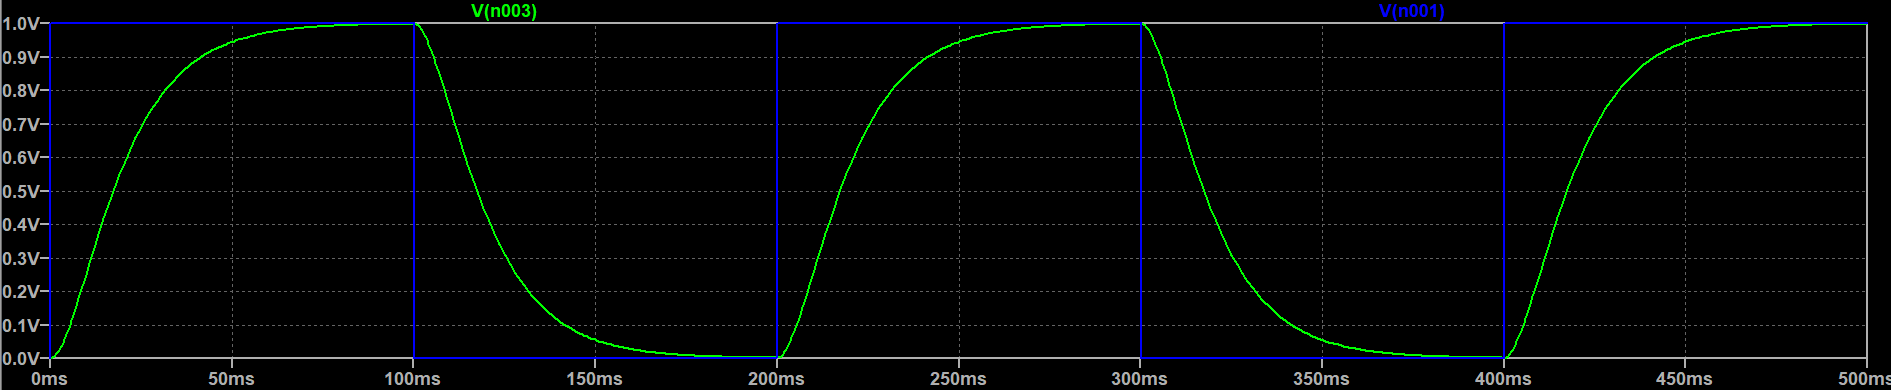
\includegraphics[width=0.9\linewidth]{Figures/Filter Waveform.png}
		\caption{Input and Output Waveform of Filter}
		\label{fig:S3}
	\end{figure}
	
	From the waveform above it can be seen that the rise time is too large, as the output (in green) is barely settling in time for the next half-cycle. This can be rectified by halving the size of the capacitors to 470nF and 47nF, as seen in Figure \ref{fig:S1}. The new output is shown in Figure \ref{fig:S4} below.
	
	\begin{figure}[h!]
		\centering
		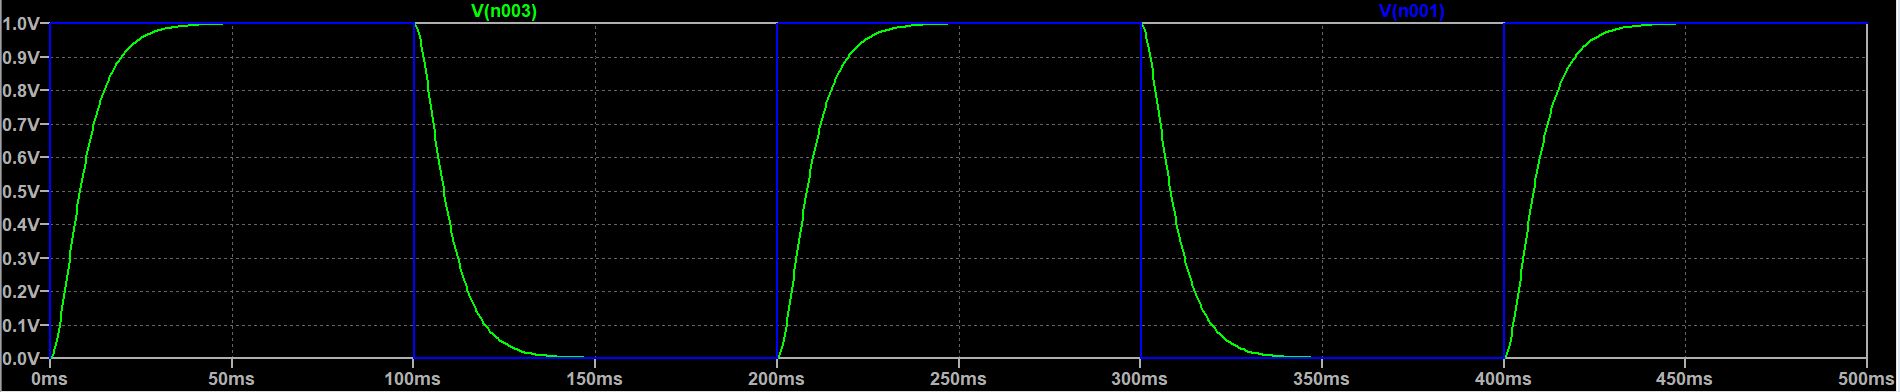
\includegraphics[width=0.9\linewidth]{Figures/Filter Waveform2.png}
		\caption{Input and Output Waveform of the Final Filter}
		\label{fig:S4}
	\end{figure}
	As seen above, the filter now meets the speed requirements.
	
	Since the instrumentation amplifier has op-amps, it needs 2 rail voltages, a positive and a negative. Unfortunately there is only a single supply, however this supply can be split in two with a simple op-amp circuit, as shown in Figure \ref{fig:S5} below.
	\begin{figure}[h!]
		\centering
		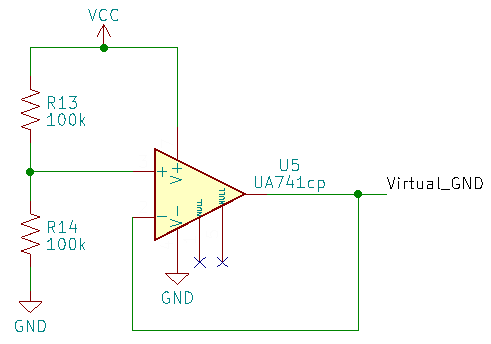
\includegraphics[width=0.5\linewidth]{Figures/Split Supply.png}
		\caption{Schematic of Split Supply Circuit}
		\label{fig:S5}
	\end{figure}
	
	If the new reference point is made to be "Virtual GND", then two rail voltages equal to $\pm \frac{V_{cc}}{2}$ are obtained. This does mean that output of the amplifier will have an offset of $\frac{V_{cc}}{2}$, but this can be stepped down using a voltage divider as to not damage the input to the microcontroller. In testing, a 5V supply was initially used but this resulted in the op-amps saturating. In the early stages of the design process, the amplifier was tested using $\pm3.3V$ and this worked fine so in the end a 6.6V supply was chosen. This will be the supply voltage required from the Power Subsystem. The Arduino Nano 33 IoT has an operating voltage of 3.3V so the voltage divider must have a gain of 0.5.
	
	Finally, because the output from the amplifier will no longer go directly to the microcontroller, an op-amp must be included in the low pass filter to buffer the input of the voltage divider. The new active low pass filter will be in a Sallen-Key configuration with $R = 100k\Omega$ and $C = 47nF$ as shown in Figure \ref{fig:S1}.
	
	\subsection{Analogue to Digital Converter (ADC)}
	Since the weight force on the load cell is proportional to output voltage out of the load cell, the change in weight is equal to the change voltage as shown in the equation below.
	\begin{center}
		$\frac{W_1}{W_2} = \frac{V_1}{V_2}$ \\ 
	\end{center}
	By substituting in the rated load, rated output and the minimum weight, the smallest change in the output can be determined.
	\begin{center}
		$\frac{0.1g}{1000g} = \frac{V_{min}}{0.5(994(3.3mV))}$ \\
		$V_{min} = 0.164mV$
	\end{center}
	As such, 1 LSB (Least Significant Bit) of ADC must be less than 0.164mV. Since the supply voltage from the Arduino is 3.3V, an ADC with a minimum resolution of 15 bits is required. The Arduino only comes with a 12-bit ADC so an external module will be needed.
	The module that was chosen is the ADS1115 16 bit ADC its specification for this application are summarized in Table \ref{tab:S4} below.
		\begin{table}[h!]
		\centering
		\caption{Table on ADS1115 specifications}
		\begin{tabularx}{0.8\textwidth} { 
				| >{\centering\arraybackslash}X 
				| >{\centering\arraybackslash}X |
				| >{\centering\arraybackslash}X |
				| >{\centering\arraybackslash}X |
				| >{\centering\arraybackslash}X |}
			\hline
			& \textbf{Min} & \textbf{Typical} & \textbf{Max} & \textbf{Unit} \\ \hline
			\textbf{Supply Voltage} & 2            & -                & 5.5          & V             \\ \hline
			\textbf{Data Rate}      & 8            & -                & 860          & SPS           \\ \hline
			\textbf{Offset error}   & -            & $\pm$ 3            & -            & LSB           \\ \hline
			\textbf{Gain error}     & -            & 0.01             & 0.15         & \%            \\ \hline
		\end{tabularx}
		\label{tab:S4}
	\end{table}
	
	From Table \ref{tab:S4}, the offset error is equivalent to 0.151mV which is less than $V_{min}$. The maximum gain error is quite large, translating to an offset of 4.95mV at the last output code. Even under typical conditions the offset will be 0.33mV. However this is not a big issue, as the scale only needs to be accurate over half the range and the gain error can be compensated for in software. The noise performance is also great as at low data rates, not a single bit of resolution is lost to quantization noise. The final reason this module was chosen is that most ADC come standalone in a SIOC package, but this one comes as a development board kit with headers allowing for easy soldering onto a Veroboard. The circuit diagram for this module is shown in Figure \ref{fig:S6} below. 
	\begin{figure}[h!]
		\centering
		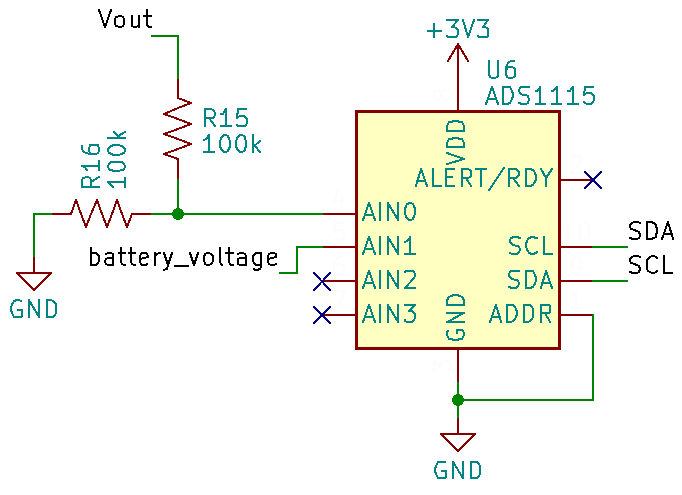
\includegraphics[width=0.4\linewidth]{Figures/ADC.png}
		\caption{Circuit Schematic of the ADS1115}
		\label{fig:S6}
	\end{figure}
	The ADC communicates with Arduino the I2C communication protocol, hence their SDA and SCL lines are connected. The Arduino has internal pull-up resistors on these lines so there's no need for external ones. The output from the amplifier is halved by the voltage divider and sent to channel 0 on the ADC. This is necessary as the ADC can only take 0.3V above the supply. In this case the supply will be the regulated 3.3V from the Arduino.
	
	\subsection{Weight Measurement Algorithm}
	The ADC was read from in code using the ADS1X15 Arduino library by Rob Tillaart \cite{ADS1115_Lib}. The ADS1115 has a programmable gain amplifier (PGA) that allows it take more precise measurements at the cost of a reduced input voltage range. The different options for the gain with corresponding full scale range and precision are shown in \ref{tab:S5} below.
	\begin{table}[h!]
		\centering
		\caption{Table on ADS1115 gain options}
		\begin{tabularx}{0.8\textwidth} { 
				| >{\centering\arraybackslash}X 
				| >{\centering\arraybackslash}X |}
			\hline
			\textbf{FSR {[}V{]}} & \textbf{LSB Size {[}uV{]}} \\ \hline
			+/- 6.144            & 187.5                      \\ \hline
			+/- 4.096            & 125                        \\ \hline
			+/- 2.048            & 62.5                       \\ \hline
			+/- 1.024            & 31.25                      \\ \hline
			+/- 0.512            & 15.625                     \\ \hline
			+/- 0.256            & 7.8125                     \\ \hline
		\end{tabularx}
		\label{tab:S5}
	\end{table}
	The second option for the gain was chosen since the input is expected to be between 1.65V and 3.3V. The LSB size for this gain also meets the accuracy requirements. The data rate was also set to 16 samples per second as the sample rate for the system will 10 samples per second. These were both set in code using the setGain() and setDataRate() functions from the library. Once setup, the sampled value would be read from the ADC using the readADC() function. The ADC value was then converted into voltage in Volts by multiplying by the value returned by the toVoltage() function. That voltage is then converted to a weight in grams using the function shown in Figure \ref{fig:S14} below. 
	\begin{figure}[h!]
		\centering
		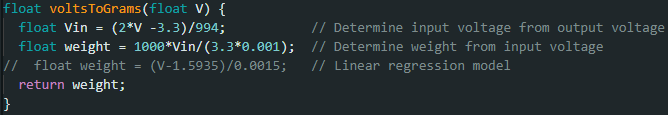
\includegraphics[width=0.8\linewidth]{Figures/voltsToGrams.png}
		\caption{Code Snippet of the Function that converts voltage to a weight}
		\label{fig:S14}
	\end{figure}
	
	The output voltage from the amplifier is given by the expression below. 
	\[V_{out} = \frac{1}{2}\left(994V_{in} + 3.3\right) \]
	The input voltage from the load cell is found from the output voltage using the expression above. The weight is then determined from the input voltage using the fact that they are proportional, and this was implemented in code as shown in \ref{fig:S14} above.
	
	The final outputted weight value was the ten-point moving average of the all the measurements. The function shown in Figure \ref{fig:S15} implements this algorithm in code.
	\begin{figure}[h!]
		\centering
		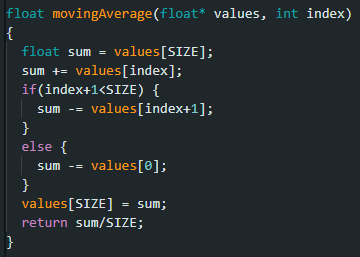
\includegraphics[width=0.5\linewidth]{Figures/MovingAverage.png}
		\caption{Code Snippet of the Function that takes the Moving Average of the weights}
		\label{fig:S15}
	\end{figure}
	If 'SIZE' is set to 10, the values array is a circular buffer that stores last 10 weight measurements, along with the sum of the whole array. The index increases incrementally with each new measurement and wraps back around to 0 once it goes past 9. This means the latest value is stored at position 'index' within the array, while the value one position ahead is the oldest. When a new value is added to the array, it is added to the sum while the oldest value is removed from the sum. The sum divided by 10 is then average that gets returned. By storing the sum in memory it removes the need for adding up all the values in the array when every measurement, making the program run more efficiently.
	
	\subsection{Tare Functionality}
	The tare function was implemented using an interrupt tied to a push button. When the button is pressed the LED is toggled, and the current weight is stored is added to an offset value. The resulting measurement will be the difference between the weight and this offset, unless the offset is larger, in which it is just 0. This was implemented in code as shown in Figure \ref{fig:S16} below.
	\begin{figure}[h!]
		\centering
		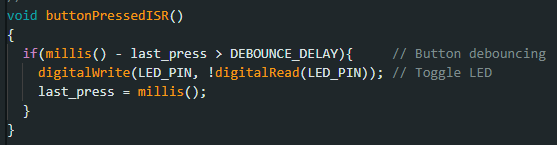
\includegraphics[width=0.7\linewidth]{Figures/ButtonPressed.png}
		\caption{Code Snippet of Interrupt Service Routine for push button}
		\label{fig:S16}
	\end{figure}
	When a button is pressed it bounces open and close many times in a split second, resulting in the microcontroller reading multiple inputs from one button press. Hence a delay of 250ms is added to allow the button to settle before taking input from it again. 
	
	\section{Acceptance Test Procedure (ATP)}
	\subsection{Load Cell and Amplifier tests}
	The amplifier circuit built on the breadboard and connected to a 6.6V power supply. The split supply was tested by measuring the voltage of the positive and negative rail with respect to "Virtual GND" using a multimeter as shown in Figure \ref{fig:S7} in Appendix A4.
	The input into the amplifier was connected to the waveform generator on the oscilloscope. The output with respect to "Virtual GND" was measured using the oscilloscope and the output with respect to GND was measured using the multimeter (this is what the ADC would measure). The input was set to 0V DC and the potentiometer was adjusted until the measured output on the oscilloscope was also 0. The output to the Arduino was then measured using a multimeter. This was repeated for different input values until the output saturated. This was compared to the ideal output given by the following expression.
	\begin{center}
		$V_{out}=\frac{1}{2}\left(994V_{in} + 3.3\right)$ \\
	\end{center}
	
	The measurement for the output when the input was 1mV DC can be seen in Figure \ref{fig:S8} in Appendix A4.
	
	The load cell was attached to a mock scale as shown in Figure \ref{fig:S9} below. Header pins were soldered to each of leads from the load cell. Within the same figure, the red and black leads were connected to $V_{cc}$ and $Virtual\_GND$ respectively, while the white and green wires leads connected to the $V_1$ and $V_2$ inputs of the amplifier respectively. A kitchen scale was then used to measure and record the weight of an empty water bottle. This bottle was then placed on the front of the scale above the nails. The output voltage from the amplifier was measured and recorded the same as before. This is shown in Figure below. This process was repeated for different weights up until the amplifier's output saturated. The weight of the bottle was varied by filling it up with different amounts of water. The bottle was placed at the same position on the scale in each run to ensure that the bottle's distance from the other end, or moment arm, was the same. 
	\begin{figure}[h!]
		\centering
		\includegraphics[width=0.8\linewidth]{Figures/Mock Scale.jpg}
		\caption{Image of mock scale}
		\label{fig:S9}
	\end{figure}
	
	\begin{figure}[h!]
		\centering
		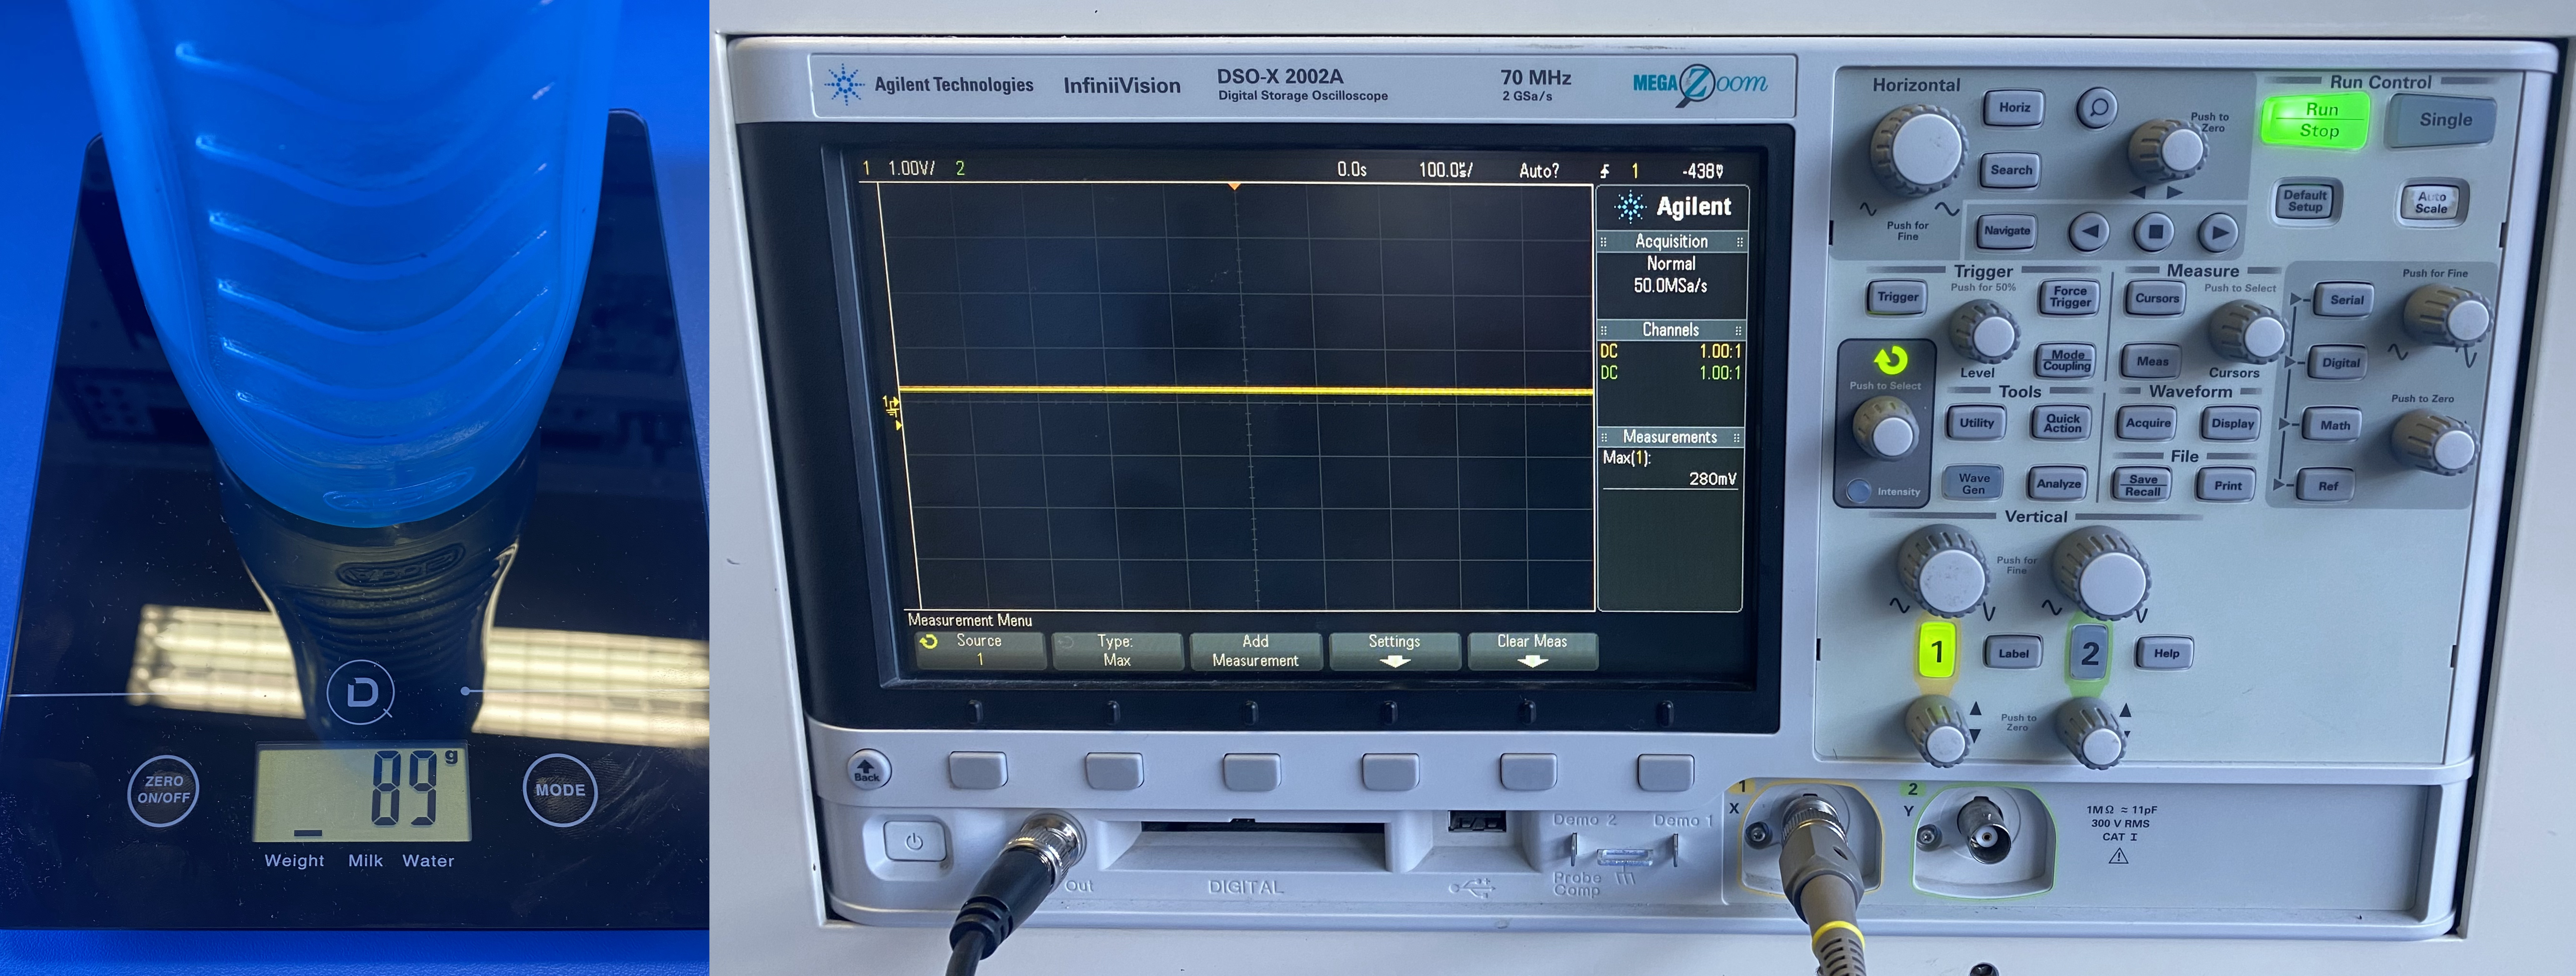
\includegraphics[width=0.8\linewidth]{Figures/ATP3.jpg}
		\caption{Image of load cell and amplifier test}
		\label{fig:S10}
	\end{figure}
	
	\subsection{Weight Measurement Test}
	The ADC was connected to the Arduino as shown in Figure \ref{fig:S6} on the breadboard. The output from the voltage divider in Figure \ref{fig:S9} was connected to channel 0 on the ADC. The Arduino was connected to the PC, the weight measurement program was run and a serial connection was established to see the output in the terminal. Once again, a bottle filled with different amounts water was placed on top of the load cell. The weight of the bottle measured by the scale and the weight measurement determined in code were both recorded. The measurement for the empty 66g bottle is shown in Figure \ref{fig:S7} below.
	\begin{figure}[h!]
		\centering
		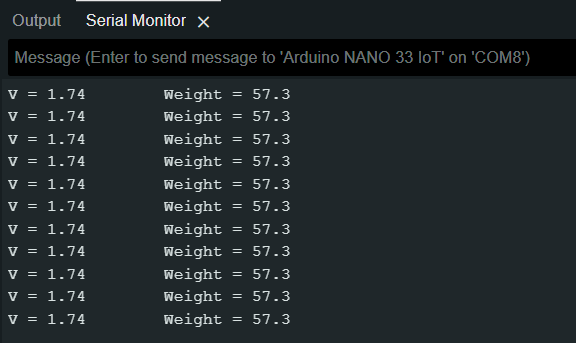
\includegraphics[width=0.6\linewidth]{Figures/Weight Measurement.png}
		\caption{Image of Weight measurement in terminal}
		\label{fig:S17}
	\end{figure}
	
	\subsection{Tare Function Test}
	The push button was now connected to pin D2 on the Arduino while the LED was placed in series with a 100 $\Omega$ resistor and connected to pin D3. The button was pressed and the resulting weight change in the terminal was observed. 
	 
	\section{Results and Discussion}
	\subsection{Load Cell and Amplifier test}
	The plot of the output voltage w.r.t. GND and "Virtual GND" against the input voltage from the oscilloscope can be found in Figure \ref{fig:S11} in Appendix A4. The plot of the output voltage against the weight is shown in Figure \ref{fig:S12} below. It can be seen that the output voltage has linear response with the weight. 
	\begin{figure}[h!]
		\centering
		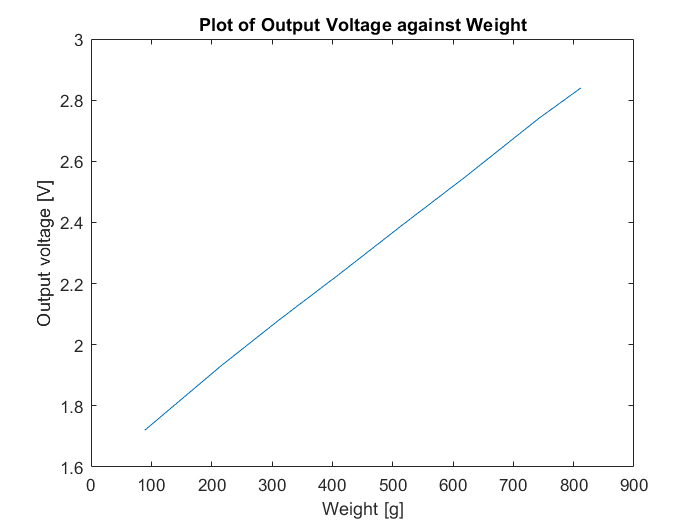
\includegraphics[width=0.4\linewidth]{Figures/Result2.png}
		\caption{Plot of the output voltage against the weight}
		\label{fig:S12}
	\end{figure}
	
	
	% ----------------------------------------------------
	\ifstandalone
	\bibliography{../Bibliography/References.bib}
	\printnoidxglossary[type=\acronymtype,nonumberlist]
	\fi
\end{document}
% ----------------------------------------------------